\documentclass[addpoints]{exam}

\makeatletter % Lagfæring fyrir nýjar útgáfur af TeXLive
\expandafter\providecommand\expandafter*\csname ver@framed.sty\endcsname
{2003/07/21 v0.8a Simulated by exam}
\makeatother

\usepackage[top=2cm, bottom=2cm, left=1cm, right=1cm]{geometry}
\usepackage[utf8]{inputenc}
\usepackage[icelandic]{babel}
\usepackage[T1]{fontenc}
%\usepackage[sc]{mathpazo}
\usepackage{helvet} \renewcommand\familydefault{\sfdefault}
\usepackage[parfill]{parskip}
\usepackage{booktabs,tabularx}
\usepackage{multirow}
\usepackage{multicol}
\usepackage{vwcol}
\usepackage{graphicx}
\usepackage{amsmath, amsfonts, amssymb, amsthm}
\usepackage{minted} %Minted and configuration
\usepackage{afterpage}
\usepackage{scrextend}

\usepackage[pdftex,bookmarks=true,colorlinks=true,pdfauthor={Eirikur Ernir Thorsteinsson},linkcolor=blue,urlcolor=blue]{hyperref}

\setcounter{secnumdepth}{-1} 
\hyphenpenalty=5000

\newcommand\blankpage{%
    \null
    \thispagestyle{empty}%
    \addtocounter{page}{-1}%
    \newpage}

\usemintedstyle{default}
\renewcommand{\theFancyVerbLine}{\sffamily \arabic{FancyVerbLine}}
\author{}
\date{}

\footer{}{}{}

\setcounter{secnumdepth}{-1} 

\qformat{\large \textbf Spurning \thequestion \phantom{M}(\totalpoints \phantom{l}stig) \hfill}
\renewcommand{\solutiontitle}{\noindent\textbf{Svar:}\par\noindent}
\renewcommand{\points}{stig}
\renewcommand{\questionshook}{\setlength{\itemsep}{0.5cm}}
\hqword{Spurning:}
\hpword{Stig í boði:}
\hsword{Stig:}
\htword{Samtals}

\title{TÖL105G Tölvunarfræði 1a - lokapróf}
\author{}
\date{18. desember 2017}

\pagestyle{headandfoot}
\firstpageheader{TÖL105G -\\ Tölvunarfræði 1a}{Lokapróf}{18. desember 2017}
\firstpagefooter{}{Bls. \thepage\ af \numpages}{}
\runningfooter{}{Bls. \thepage\ af \numpages}{}
\setlength{\columnsep}{0.5cm}

\changefontsizes{14pt}

% \printanswers
\begin{document}

% \thispagestyle{empty}
Fullt nafn: \vspace*{1mm} \hrule
\vspace*{0.5cm}

\begin{center}
\begin{minipage}{.8\textwidth}
Á þessu prófi eru \numquestions\ spurningar sem samtals gefa \numpoints\ stig.

Skrifið svör á þessar síður, ekki nota prófbók sé hún gefin.

Leyfileg hjálpargögn eru reiknivél og ein A4 blaðsíða af glósum.
\end{minipage}
\end{center}

\vspace{1cm}

\begin{questions}

\question Krossaspurningar. Merkið vandlega við réttan möguleika. 

Ekki er dregið frá fyrir röng svör.

\begin{parts}
\part[3] Gefin er skipunin
\begin{minted}{matlab}
>> x = '1' < 1;
\end{minted}
í Matlab-skipanaglugganum. Af hvaða tagi verður breytan \texttt{x}?

\begin{oneparcheckboxes}
    \choice \texttt{int32}
    \choice \texttt{double}
    \CorrectChoice \texttt{logical}
    \choice \texttt{char}
    \choice Matlab gefur villu.
\end{oneparcheckboxes}

\part[3] Gefin er skipunin 

\begin{minted}{matlab}
>> y = 3 > 2 > 1   
\end{minted}
í Matlab-skipanaglugganum. Hvert verður gildi breytunnar \texttt{y}?

\begin{oneparcheckboxes}
    \CorrectChoice \texttt{0}
    \choice \texttt{1}
    \choice \texttt{[0 1]}
    \choice \texttt{[1 0]}
    \choice Matlab gefur villu.
\end{oneparcheckboxes}



\part[3] Hversu oft keyrir lykkjan í forritinu til hliðar?
\begin{multicols}{2}
\begin{checkboxes}
\choice Aldrei
\choice Einu sinni
\CorrectChoice Fjórum sinnum
\choice Átta sinnum
\choice Óendanlega oft
\end{checkboxes}

\begin{minipage}{0.8\linewidth}
\begin{minted}[frame=lines]{matlab}
x = 1;
while x < 16
    disp('Lykkjan keyrði!')
    x = x*2;
end
\end{minted}
\end{minipage}
\end{multicols}

\part[3] Hvert af eftirfarandi gagnatögum geymir fleytitölur í Matlab?

\begin{oneparcheckboxes}
    \choice \texttt{int32}
    \CorrectChoice \texttt{double}
    \choice \texttt{logical}
    \choice \texttt{char}
    \choice \texttt{float}
\end{oneparcheckboxes}

\vspace*{1.5cm}
\hspace{0.8cm}
\gradetable[h][questions]


\part[3] Gefinn er hólfavigur:
\begin{minted}{matlab}
c = {1, 2, {3, 4, [5, 6]}};
\end{minted}
Hver eftirfarandi skipana skilar gildinu 5?

\begin{checkboxes}
    \choice \verb|c(3){3}{1}|
    \choice \verb|c{3}(3){1}|
    \choice \verb|c(3)(3){1}|
    \choice \verb|c{3}(3)(1)|
    \CorrectChoice \verb|c{3}{3}(1)|
\end{checkboxes}

\part[3] Hver eftirfarandi skipana býr til færslubreytuna \texttt{persona} með sviðið \texttt{nafn} og gildið \texttt{'Gunna'}?

\begin{checkboxes}
    \choice \verb|persona = persona.nafn('Gunna')|
    \CorrectChoice \verb|persona.nafn = 'Gunna'|
    \choice \verb|persona = struct('Gunna','nafn')|
    \choice \verb|struct(persona, 'Gunna', 'nafn')|
    \choice \verb|persona(nafn) = 'Gunna'|
\end{checkboxes}

\part[3] Ef vigrarnir $x$ og $y$ innihalda hnit 10 punkta, hvaða skipun gefur jöfnu bestu 2. stigs margliðu sem nálgar punktana?
\begin{checkboxes}
\choice \texttt{polyval(x,y,2)}
\choice \texttt{polyfit(x,y,'parabola')}
\choice \texttt{interp2(x,y,2)}
\CorrectChoice \texttt{polyfit(x,y,2)}
\choice \texttt{interp1(x,y,2)}
\end{checkboxes}

\part[3] Hver eftirfarandi skipana í Matlab skilar rökgildinu \texttt{1} þegar strengurinn \texttt{s} er \texttt{'abc'}?

\begin{checkboxes}
    \choice \texttt{s = 'abc'}
    \choice \texttt{s == 'abc'}
    \choice \texttt{s.equals('abc')}
    \choice \texttt{compare(s,'abc')}
    \CorrectChoice \texttt{strcmp(s,'abc')}
\end{checkboxes}

\part[3] Hverju skilar \texttt{nargin} inni í falli?

\begin{checkboxes}
    \CorrectChoice Heildarfjölda inntaksbreyta
    \choice Hólfavigri af inntaksbreytum
    \choice Hólfavigri af útttaksbreytum
    \choice Lengd vigursins \texttt{varargin}
    \choice Það sama og \texttt{varargin}
\end{checkboxes}

\part[3] Í Matlab er hægt að skilgreina fall í einni skipun sem\ldots

\begin{checkboxes}
    \CorrectChoice Nafnlaust fall (e. \emph{anonymous function})
    \choice Endurkvæmt fall (e. \emph{recursive function})
    \choice Hreiðrað fall (e. \emph{nested function})
    \choice Fallsfall (e. \emph{function function})
    \choice Vigurfall (e. \emph{vector function})
\end{checkboxes}

\end{parts}

\question Skrifið Matlab-skipanir (ein í hverjum lið) til að framkvæma eftirfarandi aðgerðir. Hver liður gefur eitt stig í stað tveggja sé hann rétt leystur en í meira en einni línu.
\begin{parts}
\part[2] Búið til $2 \times 4$ fylkið \texttt{m}, sem inniheldur jafndreifðar slembikommutölur á bilinu $]-3;3[$.
\vspace*{1.5cm}
\part[2] Búið til breytuna $a$ sem inniheldur meðaltal allra staka í $m$.
\vspace*{1.5cm}
\part[2] Búið til $2 \times 4$ rökfylkið \texttt{lm} sem inniheldur rökgildið ``satt'' þar sem tölugildi tilsvarandi staks í \texttt{m} er stærra en 2.
\vspace*{1.5cm}
\part[2] Breytið \texttt{m} í $4 \times 4$ fylki með því að skeyta afriti af fylkinu neðan á sjálft sig. (Þannig yrðu línur 1 og 3 alveg eins, sem og línur 2 og 4.)
\vspace*{1.5cm}
\part[2] Eyðið aftasta dálkinum úr \texttt{m}.
\ifprintanswers
\else
\vspace*{3cm}
\fi
\end{parts}

\begin{solution}
\begin{verbatim}
>> m = rand(2,4)*(3-(-3))-3;
>> a = sum(sum(m))/numel(m);
>> lm = abs(m) > 2;
>> m = [m ; m];
>> m(:,end) = [];
\end{verbatim}
\end{solution}

\newpage

\question[10] 

\begin{multicols}{2}
Skrifið Matlab-forrit sem biður notanda um að slá inn tölu og skrifar út tilsvarandi fjölda lína í þríhyrningnum til hliðar, sem inniheldur jákvæðu heiltölurnar í hækkandi röð. Þríhyrningurinn skal halda lögun sinni a.m.k. fyrstu 99 tölurnar.
\begin{verbatim}
      >> trianglenumbers
      Sláið inn tölu: 6
       1 
       2  3 
       4  5  6 
       7  8  9 10 
      11 12 13 14 15 
      16 17 18 19 20 21
\end{verbatim}
\end{multicols}

\newpage

\question[10]

\begin{multicols}{2}
Gefin er skráin \texttt{hiti.dat}, sem er á sniði sem sjá má hér til hliðar. Fyrri dálkurinn inniheldur ártal, sá seinni meðalhita á því ári í desember. 

Skrifið Matlab-skipanir sem lesa inn upplýsingarnar í skránni og teikna þær upp með ártölin á lárétta ásnum og hitastigið á þeim lóðrétta.

\begin{verbatim}
    
    
        2016 3.6
        2013 -0.5 
        2010 0.7
        2007 1.3
        ...  ...
    
    
\end{verbatim}
\end{multicols}

\begin{solution}
\begin{minted}[frame=lines] {matlab}
fid = fopen('arshiti.dat');
if fid ~= -1
    c = textscan(fid, '%f %f');
    ar = c{1};
    desemberhiti = c{2};
    plot(ar,desemberhiti);
end
fclose(fid);
\end{minted}
\end{solution}

\newpage

\question[10] Skrifið endurkvæma fallið \texttt{recrev} sem tekur inn línuvigur og skilar vigri þar sem röð stakanna hefur verið snúið við.

Dæmi um keyrslu:
\begin{verbatim}
>> recrev([1 2 3 4 5])
ans =
        5     4     3     2     1
\end{verbatim}

Fallið skal vinna með því að kalla á sjálft sig. Að hámarki helmingur stiga fæst fyrir lausn sem gerir það ekki.

\paragraph{Ábending:} Þegar vigur er af lengdinni 1 eða styttri þarf ekkert að gera til að snúa honum við. Þegar hann er af lengdinni 2 eða hærri má snúa honum við með því að skipta á staðsetningu fremsta og síðasta staksins og kalla svo á sama fall fyrir restina.

\begin{solution}
\begin{minted}{matlab}
function r = recrev(v)
if length(v) <= 1
    r = v;
else
    r = [v(end) recrev(v(2:end-1)) v(1)];
end
end
\end{minted}    
\end{solution}

\newpage

\question[10]

\begin{multicols}{2}
Efni sem eru hættuleg heilsu eru merkt með svörtum krossi á appelsínugulan bakgrunn. Skrifið Matlab-skipanir sem teikna þetta merki.

Hnitakerfiskvarðarnir gefa hugmynd um heppileg hnit til teiknunar.

Appelsínugulan má búa til með 1 hlut rauðs á móti 0.5 hlutum græns á móti 0 hlutum blás.

\begin{center}
    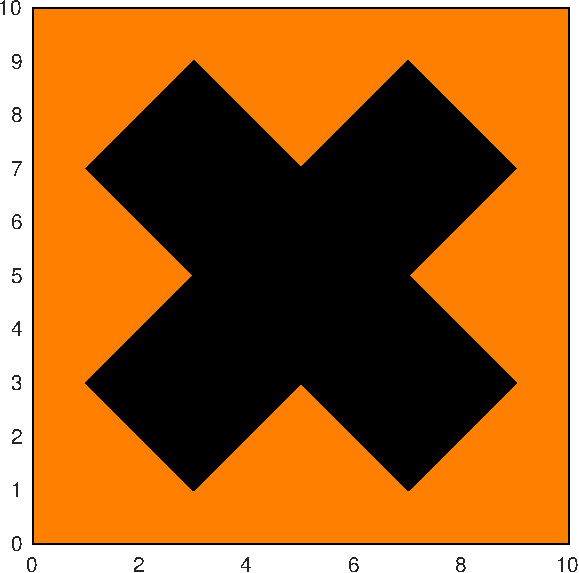
\includegraphics[width=0.8\linewidth]{Pics/haettulegtheilsu}
\end{center}

\end{multicols}

\newpage

\question[10] Búið til Matlab-klasann \texttt{Product} fyrir vörutegund sem seld er eftir vigt. Klasinn skal hafa eiginleikana \texttt{name} (t.d. ``mandarínur''), \texttt{priceperkg} og \texttt{unitsize} (t.d. 0.5 kg). Látið klasann hafa smið og tvær aðferðir til viðbótar - \texttt{unitprice} sem skilar verði á einni pakkningu og \texttt{increaseprice} sem hækkar kílóverðið um \texttt{p} prósent.

\begin{solution}
    
\begin{minted}[frame=lines]{matlab}
classdef Product
    properties
        productname
        priceperkg
        unitsize
    end
    
    methods
        
        function p = Product(name, ppkg, unitsize)
            p.productname = name;
            p.priceperkg = ppkg;
            p.unitsize = unitsize;
        end
        
        function price = packageprice(p)
            price = p.priceperkg * p.unitsize;
        end
        
        function p = increaseprice(p, increase)
            p.priceperkg = p.pricepekg*(1+increase);
        end
        
    end
end
\end{minted}
   
\end{solution}

\newpage

\question[10] Hægt er að nálga ákveðin heildi með reglu sem nefnd er trapisuregla. Í henni felst að skipta bilinu $[a,b]$ upp í $n$ jafn stór hlutbil og reikna út flatarmál trapisu yfir hvert hlutbil. Sé hlutbilslengdin $h = (b-a)/n$ og bilmörkin í $x_i=a+ih$ með $i = 1,2,\ldots,n-1$ er reglan eftirfarandi:

\[
    \int_a^b f(x) dx \approx \frac{h}{2}\left(f(a) + 2f(x_1) + 2f(x_2) + \ldots + 2f(x_{n-1}) + f(b)\right)
\]

Skrifið fall sem tekur inn $f$ (sem fallshandfang), $a$, $b$ og $n$ og reiknar heildi samkvæmt trapisureglu.

\end{questions}
\end{document}